%!TeX root = main.tex
%!encoding = UTF-8 Unicode
\section{Influence of MOSFET Parameters}
\label{sec:MR_MOSFET}

This section examines the influence of parameters that are determined by the device engineer during MOSFET design, namely the active chip area and the SiC technology generation.
Both parameters directly affect the device's parasitic capacitances and the resulting switching trajectory, so unlike the external parameters discussed in Section~\ref{sec:MR_External}, they cannot be tuned by the application engineer once a device has been selected.
For each parameter, a comparison is performed while the switching losses are kept constant, so that the differences observed in the frequency-domain spectra can be attributed to the parameter itself rather than to a shift in the switching trajectory.

\subsection{Active Chip Area}


\begin{figure}[ht]
	\centering
	\begin{subfigure}[t]{\textwidth}
		\centering
		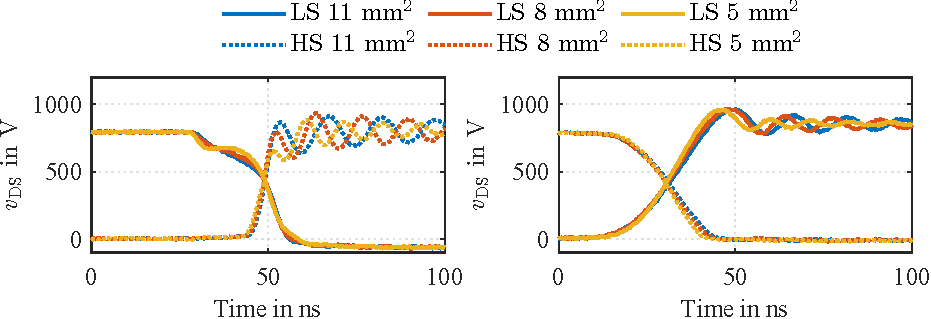
\includegraphics[scale = 1]{figures/7_MeasurementResults/MR_A_constE/MR_A_constE_Voltage_TD.pdf}
		\subcaption{Time-domain voltage measurement results.}
		\label{fig:MR_A_constE_Sweep_Voltage_TD}
	\end{subfigure} 
    
	\vspace{0.5cm}	
	
    \begin{subfigure}[t]{\textwidth}
		\centering
		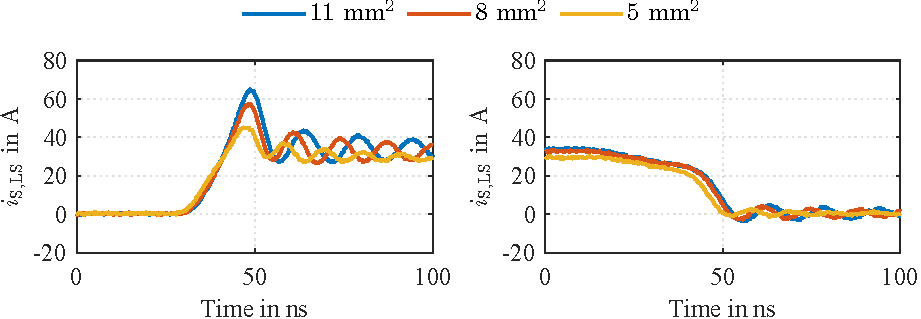
\includegraphics[scale = 1]{figures/7_MeasurementResults/MR_A_constE/MR_A_constE_Current_TD.pdf}
		\subcaption{Time-domain current measurement results.}
		\label{fig:MR_A_constE_Sweep_Current_TD}
	\end{subfigure}
	\caption{Time-domain results of the negative gate-driver bias sweep.}
\end{figure}

\begin{figure}[ht]
	\centering
	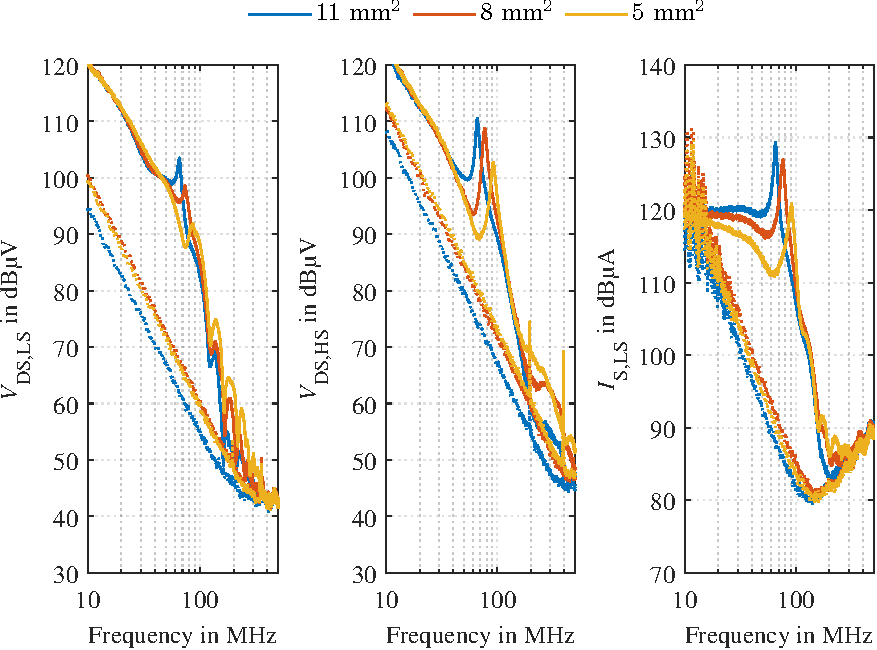
\includegraphics[scale = 1]{figures/7_MeasurementResults/MR_A_constE/MR_A_constE_FD.pdf}
	\caption{Frequency-domain measurement results of negative gate-driver bias sweep.}\label{fig:MR_A_constE_Sweep_FD}
\end{figure}


\begin{figure}[ht]
	\centering
	\begin{subfigure}[t]{\textwidth}
		\centering
		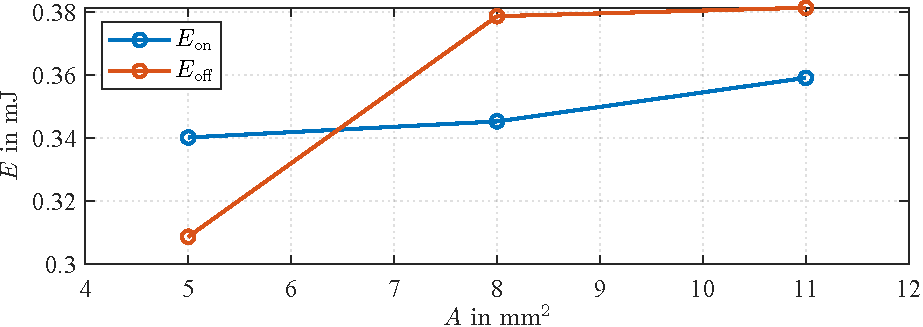
\includegraphics[scale = 1]{figures/7_MeasurementResults/MR_A_constE/MR_A_constE_Losses.pdf}
		\subcaption{Influence of negative gate-driver bias and switching losses on the EM emissions.}
		\label{fig:MR_A_constE_EmissionOverLosses}
	\end{subfigure} 

	\vspace{0.5cm}
	
    \begin{subfigure}[t]{\textwidth}
		\centering
		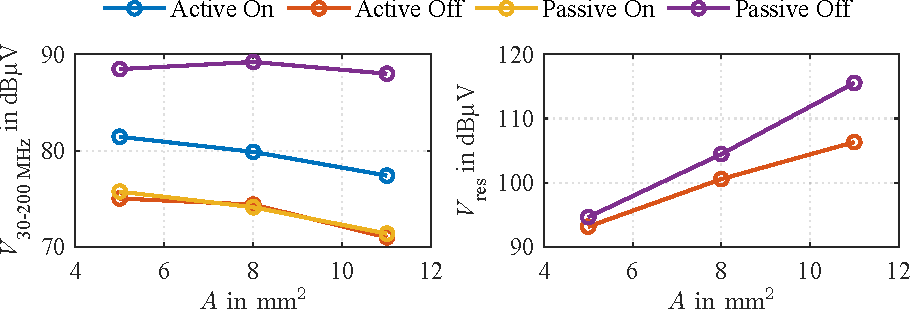
\includegraphics[scale = 1]{figures/7_MeasurementResults/MR_A_constE/MR_A_constE_Emission.pdf}
		\subcaption{EM emissions separated for turn-on and turn-off.}
		\label{fig:MR_A_constE_Emission}
	\end{subfigure}
	\caption{Negative gate-driver-bias-dependent emission and loss analysis.}
\end{figure}



\subsection{SiC Technology Generation}

\begin{figure}[ht]
	\centering
	\begin{subfigure}[t]{\textwidth}
		\centering
		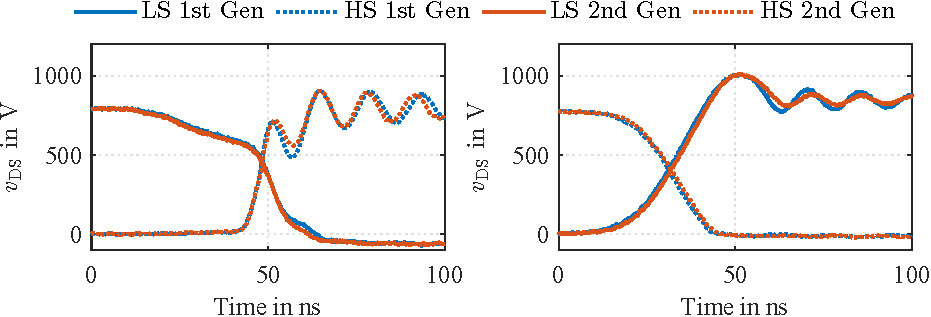
\includegraphics[scale = 1]{figures/7_MeasurementResults/MR_Gen_constE/MR_Gen_constE_Voltage_TD.pdf}
		\subcaption{Time-domain voltage measurement results.}
		\label{fig:MR_Gen_constE_Sweep_Voltage_TD}
	\end{subfigure} 
    
	\vspace{0.5cm}	
	
    \begin{subfigure}[t]{\textwidth}
		\centering
		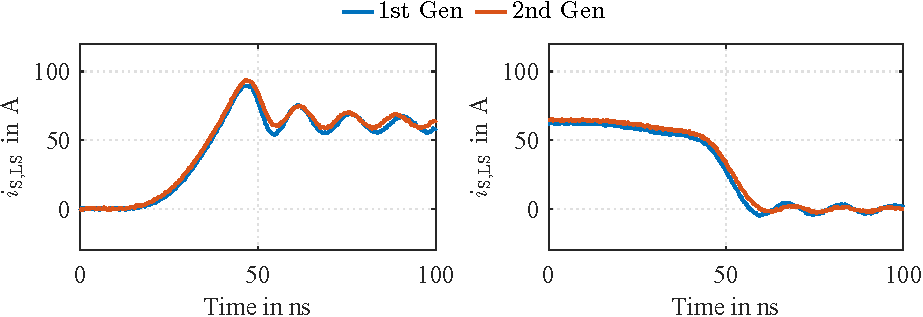
\includegraphics[scale = 1]{figures/7_MeasurementResults/MR_Gen_constE/MR_Gen_constE_Current_TD.pdf}
		\subcaption{Time-domain current measurement results.}
		\label{fig:MR_Gen_constE_Sweep_Current_TD}
	\end{subfigure}
	\caption{Time-domain results of the negative gate-driver bias sweep.}
\end{figure}

\begin{figure}[ht]
	\centering
	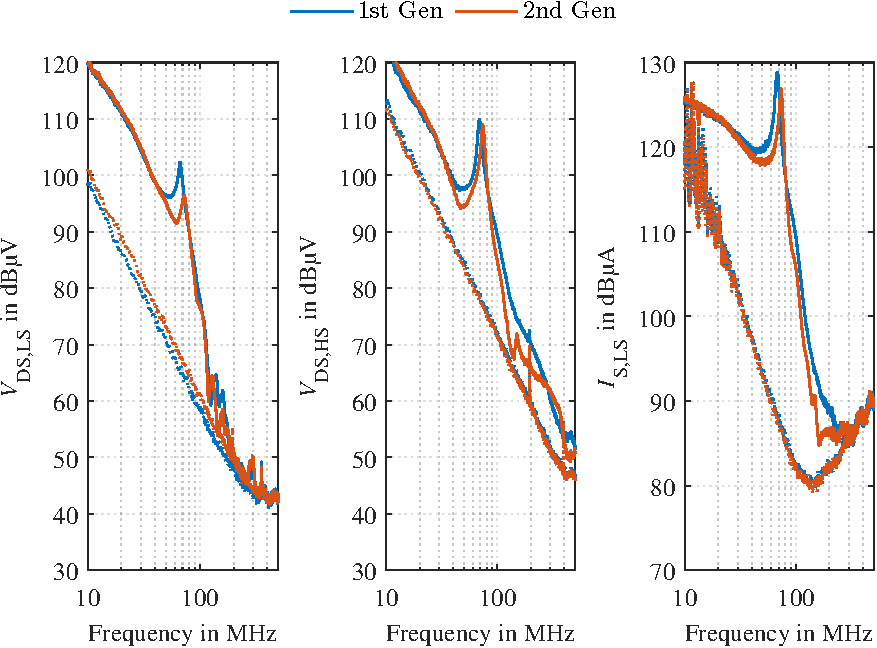
\includegraphics[scale = 1]{figures/7_MeasurementResults/MR_Gen_constE/MR_Gen_constE_FD.pdf}
	\caption{Frequency-domain measurement results of negative gate-driver bias sweep.}\label{fig:MR_Gen_constE_Sweep_FD}
\end{figure}


\begin{figure}[ht]
	\centering
	\begin{subfigure}[t]{\textwidth}
		\centering
		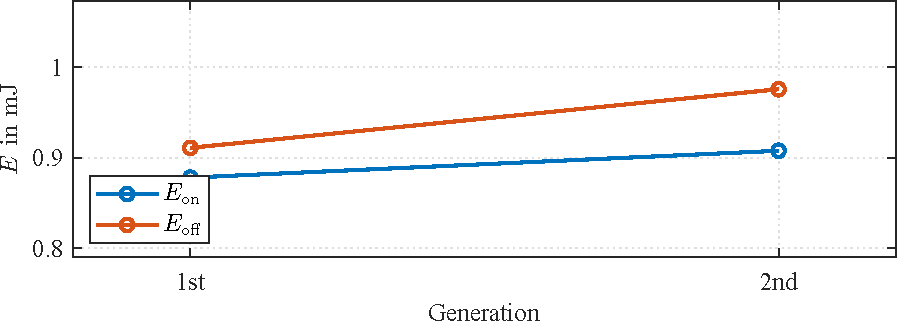
\includegraphics[scale = 1]{figures/7_MeasurementResults/MR_Gen_constE/MR_Gen_constE_Losses.pdf}
		\subcaption{Influence of negative gate-driver bias and switching losses on the EM emissions.}
		\label{fig:MR_Gen_constE_EmissionOverLosses}
	\end{subfigure} 

	\vspace{0.5cm}
	
    \begin{subfigure}[t]{\textwidth}
		\centering
		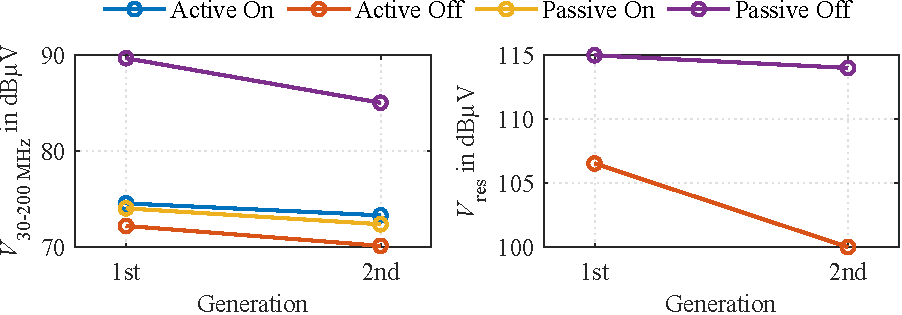
\includegraphics[scale = 1]{figures/7_MeasurementResults/MR_Gen_constE/MR_Gen_constE_Emission.pdf}
		\subcaption{EM emissions separated for turn-on and turn-off.}
		\label{fig:MR_Gen_constE_Emission}
	\end{subfigure}
	\caption{Negative gate-driver-bias-dependent emission and loss analysis.}
\end{figure}



\subsection*{Benchmarking of SiC MOSFET Manufacturers}

Beyond device-parameter studies, the proposed measurement environment also enables benchmarking of semiconductor technologies.
To demonstrate this capability and to establish EM emission as a design dimension in addition to classical trade-offs, a comparative market analysis of four SiC MOSFET devices from different manufacturers is presented.

All evaluated devices are \SI{1200}{V} SiC MOSFETs in D2PAK packages with a current rating of $\SI{60}{A}\pm\SI{5}{A}$ and are operated at $\mi{V}{DC}~=~\SI{800}{V}$ and $\mi{I}{L}~=~\SI{60}{A}$ at room temperature.

\begin{figure}[h]
	\centering
	% \includegraphics[scale = 1]{MeasurementResults/MR_MarketOverview}
	\input{7_MeasurementResults/MR_MarketOverview.tex}
	\caption{Comparative analysis of EM noise emission performance for SiC MOSFETs from different manufacturers.}\label{fig:MR_CompetitorAnalysis}
\end{figure}

Because a fair comparison at a single operating point is difficult, a gate-resistance sweep of $\mbox{\mi{R}{G,ext} = [1, 5, 10, 20, 30, 50]~\si{\ohm}}$ is performed, with an overvoltage limit of \SI{1200}{V} as the stopping criterion.
% Therefore, a gate-resistance sweep of $\mi{R}{G} = [1, 5, 10, 20, 30, 50]~\si{\ohm}$ is performed, with an overvoltage limit of \SI{1200}{V} as the stopping criterion.
The gate resistance sweep visualizes the trade-off between switching losses and EM noise emission for a given technology.
Hence, for each operating point, the switching loss energy \mi{E}{sw,tot} is calculated together with the average spectral emission of the active and passive switch voltages~\cite{kragl_impact_2024}:

% \begin{equation}
% 	\bar{V}_\mathrm{20-300MHz}^\mathrm{LS,HS} = 20 \log_{10}\left(\frac{\Delta\mi{f}{bin}\sum\limits_{\SI{20}{MHz}}^{\SI{300}{MHz}} \left(\mi{V}{DS,LS}[n] + \mi{V}{DS,HS}[n]\right)}{2\cdot(\SI{300}{MHz} - \SI{20}{MHz})\cdot\SI{1}{\micro V}}\right) 
% \end{equation}

\begin{equation}
	\bar{V}_\mathrm{20-300MHz}^\mathrm{LS,HS} = 20 \log_{10}\frac{\Delta\mi{f}{bin}\sum\limits_{\SI{20}{MHz}}^{\SI{300}{MHz}} \left(\mi{V}{DS,LS}[n] + \mi{V}{DS,HS}[n]\right)}{2\cdot(\SI{300}{MHz} - \SI{20}{MHz})\cdot\SI{1}{\micro V}}
\end{equation}


The resulting comparison, plotted in \fref{fig:MR_CompetitorAnalysis}, shows a clear and expected trend of increasing EM noise emission with decreasing switching energy.
However, the results also show that different devices emit up to \SI{7}{dB} higher average noise levels, with significantly higher differences at specific frequencies.
This establishes EM noise as a design dimension alongside classical trade-offs, and demonstrates the capability of the introduced measurement environment.

